\chapter{Hiện thực mô hình}

\begin{figure}[h!]
		\centering
		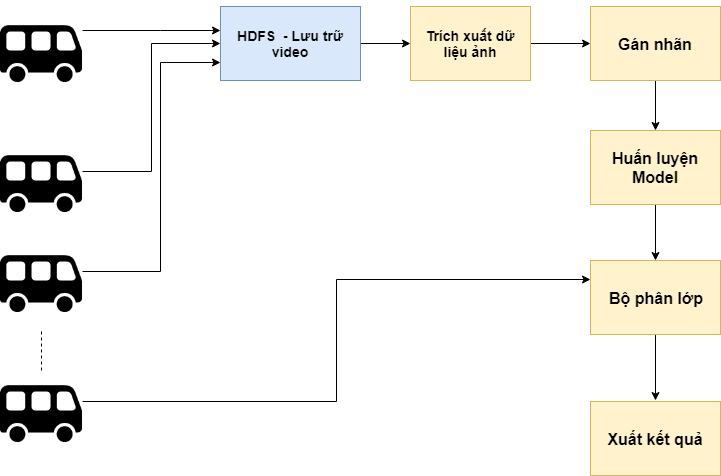
\includegraphics[scale=0.5]{charts/usecase.png}
		\caption{Mô hình phân loại ảnh giao thông kết hợp Hadoop}
		\label{fig:usecase}
	\end{figure}

\section{Tổng quan các bước}
	Hệ thống phân loại ảnh kết hợp Apache Hadoop và mô hình học sâu Deeplearning sẽ được thực hiện dựa trên sơ đồ trên. Hiện nay, các xe buýt đều được trang bị camera hanh trình và hệ thống GPS. Các video được ghi lại sẽ được lưu tại một nơi. Do số lượng của các video được gửi về liên tục và hàng ngày và giờ, nên việc sử dụng hệ thống lưu trữ HDFS của Apache Hadoop là lựa chọn hợp lý. Tiếp đến là việc truy xuất ảnh từ video và gán nhãn ảnh phục vụ cho việc huấn luyện mô hình học sâu. Đây cũng là công đoạn tốn kém chi phí nhất. Sau cùng là việc huấn luyện tập dữ liệu đã xây dựng.

\section{Các bước chuẩn bị}
\subsection{Chuẩn bị môi trường hiện thực}
	Bộ phân loại ảnh giảo hông được huấn luyện trên nền tảng hệ điều hành Linux, ngôn ngữ Python phiên bản 3.6 kết hợp với thư viện Tensorflow mã nguồn mở chuyên được sử dụng cho những mô hình học sâu.\par
	Tensorflow\cite{tf} là một thư viện học sâu mã nguồn mở được Google phát triển. Thư viện này đã thu hút được sự chú ý lớn từ cộng đồng Deep-learning. Tensorflow cho phép chạy các thuật toán machine learning trên nhiều GPU, có nhiều module được dựng sẵn giúp cho việc xây dựng và thực thi mô hình đơn giản hơn. \par
	\textbf{Các khái niệm:}
	\begin{itemize}
		\item \textbf{Tensor:} đây là cấu trúc dữ liệu được sử dụng hoàn toàn trong Tensorflow. Hay nói cách khác, tất cả dữ liệu đều biểu diễn dưới dạng tensor. Đơn giản, tensor là một mảng gồm n chiều hay list kèm theo một số thuộc tính khác.
		
		\item \textbf{Rank:} còn được gọi là số chiều của dữ liệu
		\begin{table}[h!]
			\centering
			\begin{tabular}{ | c | c | c | }
 			\hline
 			 \textbf{Rank} & \textbf{Đơn vị số} & \textbf{Ví dụ}\\
 			\hline
 			0  & Scalar  & s = 123  \\
			\hline
			1 & Vector & s = [0.8, 0.1, 0.1]	\\
			\hline
			2 & Matrix & s = [[1,2,3], [4,5,6], [7,8,9]]	\\
			\hline
			3 & 3-Tensor & s = [ [ [1], [2], [3] ], [ [4], [5], [6] ], [ [7], [8], [9] ] ]	\\
			\hline
			n & n-Tensor & n chiều dữ liệu... \\
			\hline
			
		\end{tabular}
		\caption{Các chiều dữ liệu.}
		\label{table:rank}
		\end{table}
		
		
		
		
		\item \textbf{Shape:} biểu diễn chiều của tensor. Ví dụ, \(t = [[1,2,3], [4,5,6], [7,8,9]]\) có shape là \([3, 3]\), \(t = [ [ [1], [2], [3] ], [ [4], [5], [6] ], [ [7], [8], [9] ] ]\) có shape là \([1, 3, 3]\),...
		
		\item \textbf{Type:} là các kiểu dữ liệu được sử dụng trong Tensorflow. Một vài kiểu dữ liệu cơ bản như.\\
		\begin{table}[h!]
			\centering
			\begin{tabular}{ | c | c | c | }
 			\hline
 			 \textbf{Data type} & \textbf{Python code} & \textbf{Mô tả}\\
 			\hline
 			\textit{DT-FLOAT}  & tf.float32  & 32 bits floating point.  \\
			\hline
			\textit{DT-DOUBLE} & tf.float64 & 64 bits floating point.\\
			\hline
			\textit{DT-INT16} & tf.int16	 & 16 bits signed integer.\\
			\hline
			\textit{DT-INT32} & tf.int32	 & 32 bits signed integer.	\\
			\hline
			\textit{DT-INT64} & tf.int64	 & 64 bits signed integer. \\
			\hline
			... & ... & ...\\
			\hline
			
		\end{tabular}
		\caption{Một vài kiểu dữ liệu.}
		\label{table:type}
		\end{table}
		\pagebreak
		
		
	\end{itemize}
	
	

\section{Các bước hiện thực}

	\subsection{Cài đặt Apache Hadoop}
	Trong phần hướng dẫn này chúng ta sẽ biết được cách cài đặt một cụm gồm nhiều máy Hadoop. Thông qua nhiều bước,ta sẽ biết cách cấu hình cũng như khởi tạo và kết thúc hoạt động của một cụm máy Hadoop.\par 
	\subsubsection{Cấu hình cần thiết để cài đặt một cụm 3 máy hadoop}
	Một cụm Hadoop có thể rất nhiều máy, nhưng để có được cái nhìn tổng quan và vì thời gian của đề tài nên chúng ta sẽ tiến hành cài Hadoop trên 3 máy tính. Việc bổ sung thêm máy trạm vào cụm sẽ được hướng dẫn ở nội dung cuối phần này.\par 
	\begin{itemize}
		\item \textbf{Số lượng máy tính: } 3 máy tính.
		\item \textbf{Hệ điều hành: } sử dụng hệ điều hành Ubuntu phiên bản 14.04 hoặc 16.04 hoặc cao hơn.
		\item \textbf{Phiên bản Apache Hadoop: }Gói cài đặt \href{http://hadoop.apache.org/releases.html}{Hadoop phiên bản 3.1.0}
	\end{itemize}
	\subsubsection{Cài đặt Hadoop trên máy Master(Namenode)}
	Mục này được thực hiện chỉ riêng trên máy được chọn làm Master.
		\begin{enumerate}
			\item \textbf{Các vấn đề trước khi cài đặt Hadoop:}
			\begin{itemize}
			
				\item \textbf{Thêm địa chỉ IP đầu vào vào file \textit{/etc/hosts}}				
				\begin{lstlisting}[caption=Nội dung file /etc/hosts]
	127.0.0.1	localhost
	127.0.1.1	master
	192.168.1.50	master
	192.168.1.61	slave
	192.168.1.73	slave1

				\end{lstlisting}
				Chúng ta bỏ qua 2 dòng đầu của file va chú ý tới 3 dòng tiếp theo. Bên cột trái, đó chính là lần lượt địa chỉ IP của 3 máy sẽ cài Hadoop. 192.168.1.50 là máy được chọn làm master và từ \textit{master} bên cột phải là hostname của máy đó. Tương tự 2 dòng cuối, đó là IP của 2 máy được chọn làm datanode và hostname lần lượt là \textit{slave, slave1}.\par 
				\item \textbf{Cài đặt Java:} hiện nay, Java được cài ở đây sẽ có phiên bản là Java 8. Thực hiện lần lượt các lệnh sau trên terminal để cài đặt Java 8.
				
				\begin{lstlisting}[language=python,caption=Cài đặt Java 8]
	sudo add-apt-repository ppa:webupd8team/java	
	sudo apt-get update	
	sudo apt-get install oracle-java8-installer
	
				\end{lstlisting}
				
				\item \textbf{Cấu hình SSH: } Thực hiện lần lượt các lệnh sau để cài cũng như cấu hình kết nối SSH máy master tới các máy datanodes.
				
				\begin{lstlisting}[caption=Cài đặt SSH]
	sudo apt-get install openssh-server openssh-client	
	ssh-keygen -t rsa -P ""	
				\end{lstlisting}
				Sao chép nội dung file .ssh/id\_rsa.pub của máy master đến file .ssh/authorized\_keys của máy master cũng như các máy datanodes. Sau đó kiểm tra kết nối đã thành công hay chưa bằng lệnh.\par
				\begin{lstlisting}[caption=Kết nối SSH]
	ssh slave
	ssh slave1
				\end{lstlisting}
				
			\end{itemize}
			\item \textbf{Cài đặt Hadoop}
			\begin{itemize}
				\item \textbf{Tải gói cài đặt: }Tải gói cài đặt Hadoop theo link phía dưới\\
				http://hadoop.apache.org/releases.html
				\item \textbf{Giải nén gói cài đặt: }Giải nén đến thu mục \textit{/usr/local} bằng câu lệnh
				\begin{lstlisting}
tar xzf hadoop-3.1.0.tar.gz -C /usr/local/
				\end{lstlisting}
				\item \textbf{Chỉnh sửa ~/.bashrc: }Thêm các biến môi trường cài đặt Hadoop vào file ~/.bashrc như nội dung sau.
		
				\begin{lstlisting}[language=bash]
export HADOOP_PREFIX="/usr/local/hadoop-3.1.0"
export PATH=$PATH:$HADOOP_PREFIX/bin
export PATH=$PATH:$HADOOP_PREFIX/sbin
export HADOOP_MAPRED_HOME=${HADOOP_PREFIX}
export HADOOP_COMMON_HOME=${HADOOP_PREFIX}
export HADOOP_HDFS_HOME=${HADOOP_PREFIX}
export YARN_HOME=${HADOOP_PREFIX}
				\end{lstlisting}
				Sau khi lưu nội dung chỉnh sửa, thưc thị \textit{source ~/.bashrc} để các biến hệ thống thiết lập các biến môi trường.
				\item \textbf{Cấu hình file hadoop-env.sh: }cấu hình biến \textit{JAVA\_HOME}
				\begin{lstlisting}[language=bash]
export JAVA_HOME=/usr/lib/jvm/java-8-oracle/
				\end{lstlisting}
				Thay đổi đường dẫn \textit{JAVA\_HOME} nếu cài đặt Java 8 ở một nơi khác.
				\item \textbf{Cấu hình file core-site.xml: }thêm các dòng sau
				\begin{lstlisting}[language=XML]
<configuration>
<property>
	<name>fs.defaultFS</name>
	<value>hdfs://master:9000</value>
</property>
<property>
	<name>hadoop.tmp.dir</name>
	<value>/home/'your\_user'/hdata</value>
</property>
</configuration>
				\end{lstlisting}
				\item \textbf{Cấu hình file hdfs-site.xml: }thêm các nội dung như sau
				\begin{lstlisting}[language=XML]
<configuration>
<property>
	<name>dfs.replication</name>
	<value>2</value>
</property>
</configuration>
				\end{lstlisting}
				\item \textbf{Cấu hình file mapred-site.xml: }thêm các nội dung như sau
				\begin{lstlisting}[language=XML]
<configuration>
<property>
	<name>mapreduce.framework.name</name>
	<value>yarn</value>
</property>
</configuration>
				\end{lstlisting}
				\item \textbf{Cấu hình yarn-set.xml: }thêm các nội dung như sau
				\begin{lstlisting}[language=XML]
<configuration>
<property>
	<name>yarn.nodemanager.aux-services</name>
	<value>mapreduce_shuffle</value>
</property>
<property>
	<name>yarn.resourcemanager.scheduler.address</name>
	<value>master:8030</value>
</property>
<property>
	<name>yarn.resourcemanager.address</name>
	<value>master:8040</value>
</property>
</configuration>
				\end{lstlisting}
				\item \textbf{Cấu hình file workers: }thêm hostname của 3 máy trạm mà đã đặt ở file \textit{/etc/hosts}
				\begin{lstlisting}
master
slave
slave1
				\end{lstlisting}
			\end{itemize}
			
			
			
		\end{enumerate}
		
		\subsubsection{Cài đặt Hadoop trên các datanodes}
		\begin{enumerate}
			\item \textbf{Các cấu hình chuẩn bị: }
			\begin{itemize}
				\item \textbf{Thêm địa chỉ IP vào file /etc/hosts: }thực hiện giống như đã làm ở máy master
				\item \textbf{Cài đặt Java 8}
			\end{itemize}
			\item \textbf{Cài đặt Hadoop cho tất cả máy datanodes: }thao tác này sẽ được thực hiện trên terminal của máy master.
			\begin{itemize}
				\item \textbf{sử dụng SSH để gửi file cài đặt: }thực hiện lần lượt các lệnh sau để gửi file cài đặt hadoop tới các máy datanodes
				\begin{lstlisting}
scp /usr/local/hadoop-3.1.0 slave:/usr/local/hadoop-3.1.0
scp /usr/local/hadoop-3.1.0 slave1:/usr/local/hadoop-3.1.0
				\end{lstlisting}
				Sau các lệnh này được thực thi xong thì các máy datanodes đã được cài đặt hadoop thành công
				\item \textbf{Cấu hình file ~/.bashrc: }chúng ta có thể copy nội dung từ file \textit{~/.bashrc} của master đến các máy datanodes.
			\end{itemize}
			
			\item \textbf{Khởi động cụm máy Hadoop: }chạy các lệnh sau để khởi động Hadoop
			\begin{itemize}
				\item \textit{bin/hdfs namenode -format}
				\item \textit{sbin/start-dfs.sh}			
			\end{itemize}
			\item \textbf{Kiểm tra xem Hadoop service:} lần lượt thực thi lệnh jps từ terminal của các máy master và datanode để kiểm tra, nếu kết quả như hình dưới đây thì các service hadoop đang hoạt động.
			\begin{figure}[h!]
				\centering
				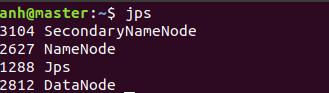
\includegraphics[scale=0.8]{charts/jps-m.png}
				\caption{Kiểm tra Hadoop service trên master}
				\label{fig:jps-m}
			\end{figure}
			\begin{figure}[h!]
				\centering
				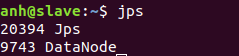
\includegraphics[scale=0.8]{charts/jps-s.png}
				\caption{Kiểm tra Hadoop service trên worker(slave)}
				\label{fig:jps-s}
			\end{figure}
			\begin{figure}[h!]
				\centering
				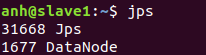
\includegraphics[scale=0.8]{charts/jps-s1.png}
				\caption{Kiểm tra Hadoop service trên worker(slave1}
				\label{fig:jps-s1}
			\end{figure}
			
			
		\end{enumerate}
		
	\subsubsection{Thêm một datanodes vào một cụm Hadoop đang hoạt động}
	Trong quá trình sử dụng, việc muốn mở rộng cụm máy Hadoop là điều có thể xảy ra. Chúng ta có thể dễ dàng thêm một datanodes và một cụm máy Hadoop đang hoạt động theo các bước sau.
	\begin{enumerate}
		\item \textbf{Cài đặt Java 8: }đảm bảo rằng máy được thêm vào cụm phải được cài đặt Java 8 như đã trình bày ở phía trên.
		\item \textbf{Thêm địa chỉ IP vào /etc/hosts: }thêm địa chỉ IP của máy datanode mới vào file /etc/hosts của máy master và các máy datanodes đã có cũng như datanode mới.
		\item \textbf{Cấu hình SSH: }copy nội dung file ~/.ssh/id\_rsa.pub vào máy datanodes mới giống như đã làm với các máy datanode đã trước.
		\item \textbf{Cài đặt Hadoop: }chúng ta cũng sử dụng SSH để gửi thư mục cài Hadoop từ máy master sang máy datanode mới như đã thực hiện.
		\item \textbf{Cấu hình file workers: }thêm hostname của máy datanode mới vào file workers trên máy master.
		\item \textbf{Khởi động datanode: }thực hiện file \textit{start-dfs.sh} trong thư mục sbin trên máy master để tiến hiện khởi động datanode mới vào cụm máy.
	\end{enumerate}
		
	\subsubsection{Lưu trữ dữ liệu ảnh trên HDFS}
	Để đưa dữ liệu lên HDFS, ta sử dụng câu lệnh sau.
	\begin{lstlisting}
hdfs dfs -put ~/Document/traffic/ hdfs://master:9000/
	\end{lstlisting}
	Với \textit{~/Document/traffic} là đương dẫn đến thư mục lưu dữ liệu ảnh, và \textit{hdfs://master:9000/} là đường dẫn đến vị trí lưu của HDFS. Để xem kết quả put ta thực hiện lệnh sau để liệt kê các thư mục dữ liệu đã được lưu trên HDFS.
	\begin{figure}[h!]
				\centering
				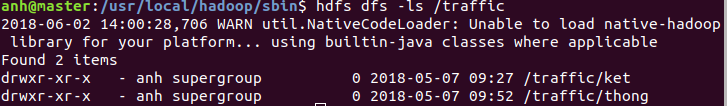
\includegraphics[scale=0.6]{charts/dfs-ls.png}
				\caption{Liệt kê thư mục dữ liệu trên HDFS}
				\label{fig:dfs-ls}
	\end{figure}
	
	\subsection{Cài đặt HIVE}
	Để cài đặt HIVE và lưu trữ dữ liệu GPS, ta thực hiện các bước sau đây.
	\subsubsection{Tải gói cài đặt HIVE}
	Tải gói cài đặt HIVE ở với đường dẫn sau \textit{http://mirror.downloadvn.com/apache/hive/}, ta sẽ sử dụng phiên bản 2.2.0.
	\subsubsection{Cài đặt HIVE}
	\begin{enumerate}
		\item \textbf{Giải nén: }giải nén gói cài đặt và copy thư mục có được vào vị trí thư mục muốn cài chẳng hạn như \textit{/usr/local/hive}.
		\item \textbf{Cấu hình biến môi trường: }thêm vào file \textit{~/.bashrc} nội dung như sau
		\begin{lstlisting}[language=bash]
export HIVE_HOME=/usr/local/hive
export PATH=$PATH:$HIVE_HOME/bin
export CLASSPATH=$CLASSPATH:/usr/local/Hadoop/lib/*:.
export CLASSPATH=$CLASSPATH:/usr/local/hive/lib/*:.
	\end{lstlisting}
	Thực hiện lệnh \textit{source ~/.bashrc} để thực thi cấu hình.
	\end{enumerate}
	
	\subsubsection{Tải và cài đặt Apache Derby}
	Làm theo các lệnh hướng dẫn để tải à cài đặt Apache Derby
	\begin{enumerate}
		\item \textbf{Tải Apache Derby: } vào và tải ở địa chỉ sau \textit{http://archive.apache.org/dist/db/derby/} với phiên bản 10.14.2.0
		\item \textbf{Giải nén: } giải nén vào thư mục \textit{/usr/local/derby}
		\item \textbf{Cấu hình biến môi trương cho Derby:} Thêm nội dung file \textit{~/.bashrc} như sau.
		\begin{lstlisting}[language=bash]
export DERBY_HOME=/usr/local/derby
export PATH=$PATH:$DERBY_HOME/bin
		\end{lstlisting}
	\end{enumerate}
		
	\subsubsection{dữ liệu GPS }
	Dữ liệu GPS là tập dữ liệu lưu vị trí GPS của một xe buýt trong một thời điểm nhất định. Dữ liệu này được lưu bằng bảng trong HIVE. Cấu trúc của bảng dữ liệu bao kinh độ, vĩ độ, thơi điểm theo định dạng DD/MM/YYYY hh:mm:ss.
	
	

	\subsection{Xử lý dữ liệu}
	
	Để xây dựng mô hình phân loại hình ảnh, chúng ta cần phải có một tập huấn luyện đủ tốt. Ở đây, các hình ảnh được trích xuất từ camera hành trình từ các tuyến xe buýt. \par
	Cấu trúc tổ chức tập dữ liệu gồm 2 thư mục chính:
	\begin{itemize}
		\item Thư mục \textbf{ket}: chứa các hình ảnh được cho là giao thông trong tình trạng ùn tắt. Bao gồm khoảng 7500 hình ảnh định dạng JPG.
		\item Thư mục \textbf{thong}: chứa các hình ảnh được cho là giao thông trong tình trạng thông tháng. Bao gồm 7700 hình ảnh định dạng JPG.
	\end{itemize}
	
		Các hình ảnh được trình bày và lưu trữ vào các thư mục có chứa các tên mô tả cho đặt tính của những hình ảnh đó. Với bộ dữ liệu trên, chương trình tạo một kiểu dữ liệu dictionary với khóa chính là giá trị biểu diễn cho tên thư mục và cũng là tên class cần phân loại, value chính là đường dẫn các file ảnh tương ứng.\par
		 Để sử dụng được trong mô hình mạng, các hình ảnh sẽ được mã hóa sang một định dạng mới nhờ các phương thức hỗ trợ có sẵn trong thư viện Tensorflow. Sau khi được mã hóa, kết quả chính là các tensor có thông số shape như sau [299, 299, 3], với hai vị trí đầu tiên chính là kích thước của hình ảnh cũng như của tensor, giá trị 3 biểu diễn cho độ sâu (ảnh màu).\par
	 	Sau cùng, bộ dữ liệu đã được mã hóa được chia thành 3 tập con sử dụng với 3 mục đích khác nhau: tập huấn luyện(Training set), tập validation để tránh vấn đề overrfit trong quá trình huấn luyện và tập kiểm thử dùng để kiểm tra độ chính xác của mô hình sau khi huấn luyện hoàn tất.	Riêng tập huấn luyện sẽ được dùng để tạo ra các bottlenecks
	
	\subsection{Tạo các bottlenecks}
	
	Bottlenecks\cite{bottlenecks} là một từ được dùng để chỉ tầng (layer) nằm ngay trước fully-connected layer. Với kiến trúc mạng googLeNet, tầng này đã được huấn luyện tập dữ liệu trước đó nên có được kết quả đủ tốt để phân biệt được đặc tính của mỗi lớp(class) yêu cầu. Có nghĩa ở bước này chúng ta sẽ tạo ra một bản tóm tắt các giá trị trọng số đủ tốt cho mỗi ảnh input. Tầng cuối cùng của kiến trúc mạng sẽ sử dụng các giá trị bottlenecks này để huấn luyện và điều chỉnh để phân loại các lớp mới. Điều này nhờ vào việc mạng đã được huấn luyện bởi tập dữ liệu gồm 1000 lớp khác nhau của ImageNet giúp cho việc phát hiện các mẫu đặc tính trở nên dễ dàng hơn.
	
	\subsection{Huấn luyện}
		
	Sau khi hoàn tất tạo các giá trị bottleneck, việc thực hiện thực hiện cấu hình mạng và huấn luyện bắt đầu. Tổng số bước huấn luyện sẽ được cài đặt mặc định là 4000 bước, tuy nhiên có thể thay đổi lại tùy theo tình huống. Mỗi bước huấn luyện sẽ chọn ra 100 dữ liệu ngẫu nhiên \footnote{Tập dữ liệu lúc này là những bottlenecks} để đưa vào tầng cuối cùng \footnote{Tầng fully-connected với softmax là activation function} để dự đoán lớp, lớp dự đoán sẽ được so sánh với các lớp thực tế để mạng điều chỉnh và cập nhật các giá trị trọng số thông qua cơ chế lan truyền ngược như đã trình bày ở chương trước. Do phép toán được thực hiện trên tập huấn luyện nên sẽ  gây ra vấn đề overfit, vì thế mà tập validation sẽ được sử dụng để đo lại giá trị sai lệch và độ chính xác. Nếu độ chính xác tại tập huấn luyện cao nhưng tại tập validation không thay đổi hoặc thấp thì chứng tỏ mô hình mạng gặp phải vấn đề overfit và việc huấn luyện tiếp tục không còn có ích.
	
	\subsection{Chạy Huấn luyện bằng cách kết hợp tensorflow với hệ thống HDFS}
	\subsubsection{Chuẩn bị}
	Ở các nội dung trên, chúng ta đã thực hiện việc cài đặt Apache Hadoop cũng như các biến môi trường cần thiết, trong đó có hai biến môi trường cần thiết để chạy thực thi mô hình trên là \textbf{JAVA\_HOME} và vị trí cài đặt Hadoop\textbf{HADOOP\_HDFS\_HOME}. Bây giờ chúng ta sẽ cần thêm một biến môi trường cho hệ thống nữa.
	\begin{itemize}
		\item \textbf{LD\_LIBRARY\_PATH: }để thêm biến này, chúng ta cần thêm vào file \textit{~/.bashrc} nội dung như sau.	
	\begin{figure}[h!]
			\centering
			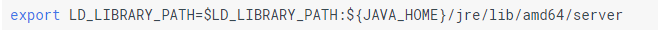
\includegraphics[scale=0.8]{charts/ldlib.png}
			\caption{Nội dung thư viện LD\_LIBRARY\_PATH}
	\end{figure}
		
	\end{itemize}
	\subsubsection{Chạy mô hình huấn luyện.}
	Chúng ta thực hiện câu lệnh sau đây để tiến hành chạy mô hình huấn luyện kết nối với tập dữ liệu ở HDFS.
	\begin{figure}[h!]
			\centering
			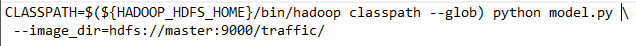
\includegraphics[scale=0.8]{charts/run.png}
			\caption{Câu lệnh thực thi huấn luyện mô hình}
	\end{figure}

